\section{Actividad 02: Creación del  paquete DTSX} 


1. Abrimos un nuevo Proyecto en nuestro Visual Studio\\
	\begin{center}
	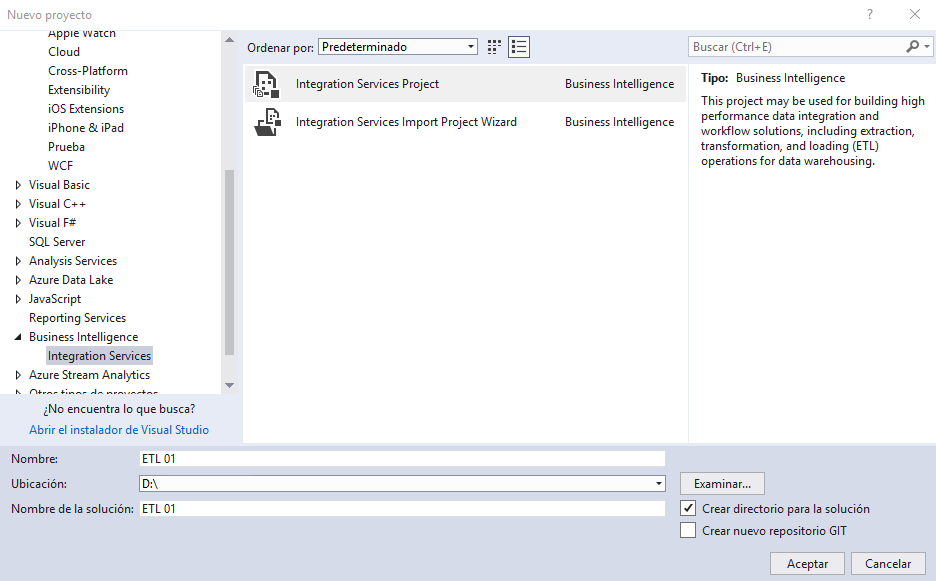
\includegraphics[width=13cm]{./Imagenes/img13}
	\end{center}	

2. En al ventana nueva, sección Solución Explorer, Agrego el paquete generado antes\\
	\begin{center}
	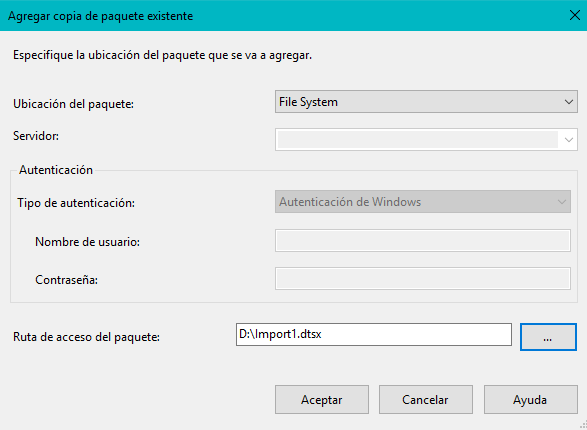
\includegraphics[width=13cm]{./Imagenes/img14}
	\end{center}	
	\begin{center}
	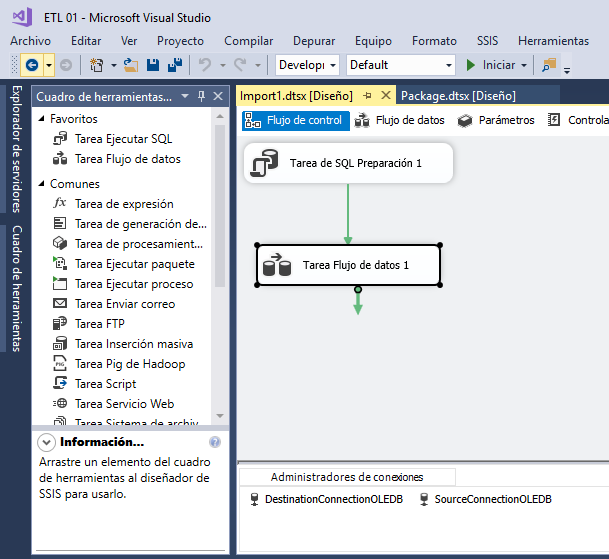
\includegraphics[width=12cm]{./Imagenes/img15}
	\end{center}	
3. Observamos las caracteristicas obtenidas.\\
	\begin{center}
	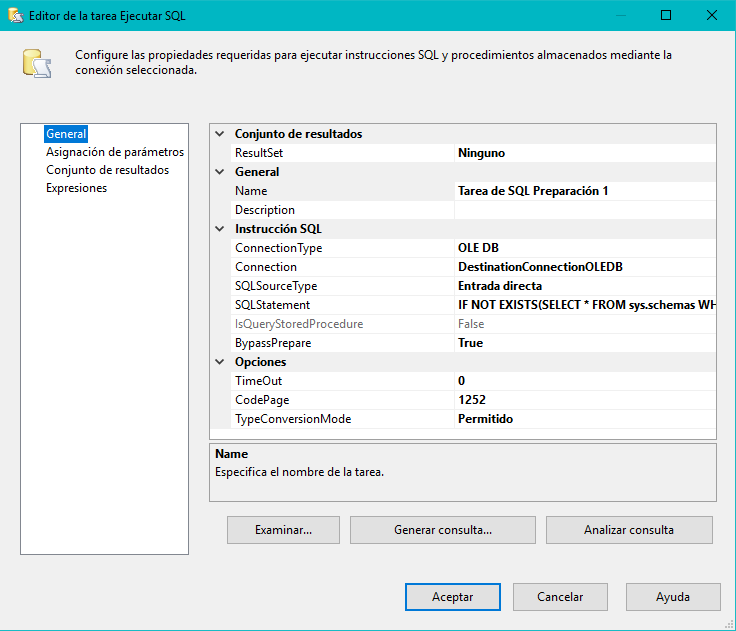
\includegraphics[width=13cm]{./Imagenes/img16}
	\end{center}	

4. En la siguiente ventana mostramos el paquete que se ha importado.\\
	\begin{center}
	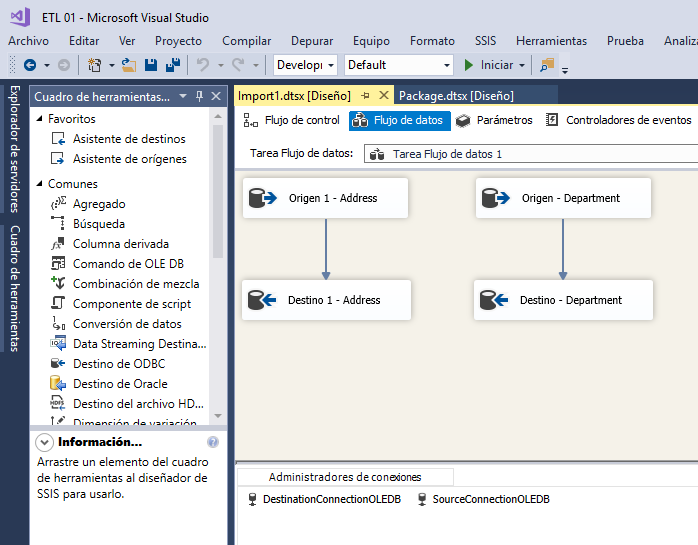
\includegraphics[width=12cm]{./Imagenes/img17}
	\end{center}	
5. Agregamos el administrador de conexiones en este caso el OLEBD. \\
	\begin{center}
	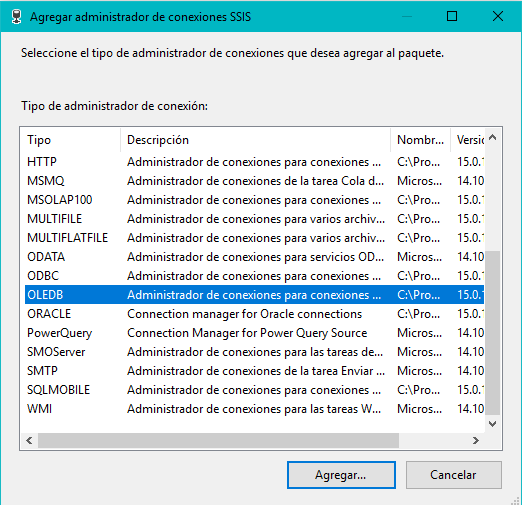
\includegraphics[width=12cm]{./Imagenes/img18}
	\end{center}	

6. En la siguiente ventana mostramos el paquete que se ha importado.\\
	\begin{center}
	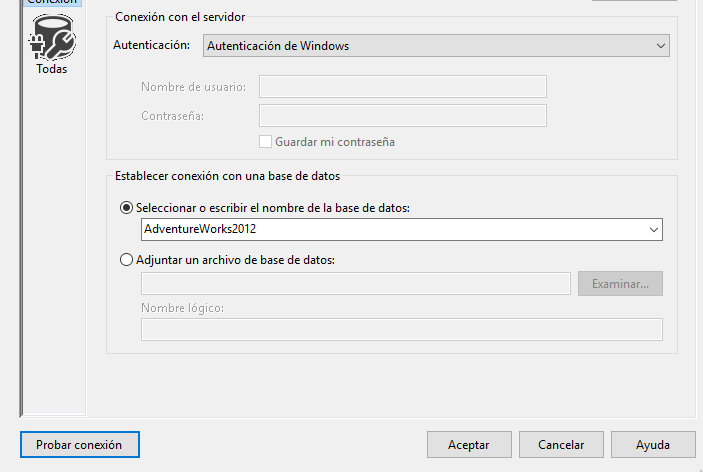
\includegraphics[width=12cm]{./Imagenes/img19}
	\end{center}	
7. Observamos las caracteristicas establecidas.\\
	\begin{center}
	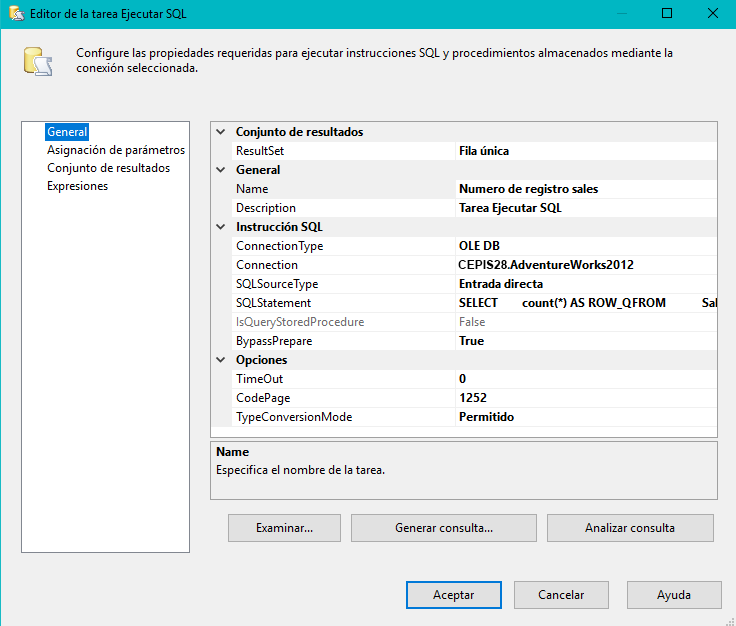
\includegraphics[width=12cm]{./Imagenes/img20}
	\end{center}	
8. Editamos el componente Scrtipt Task Editor.\\
	\begin{center}
	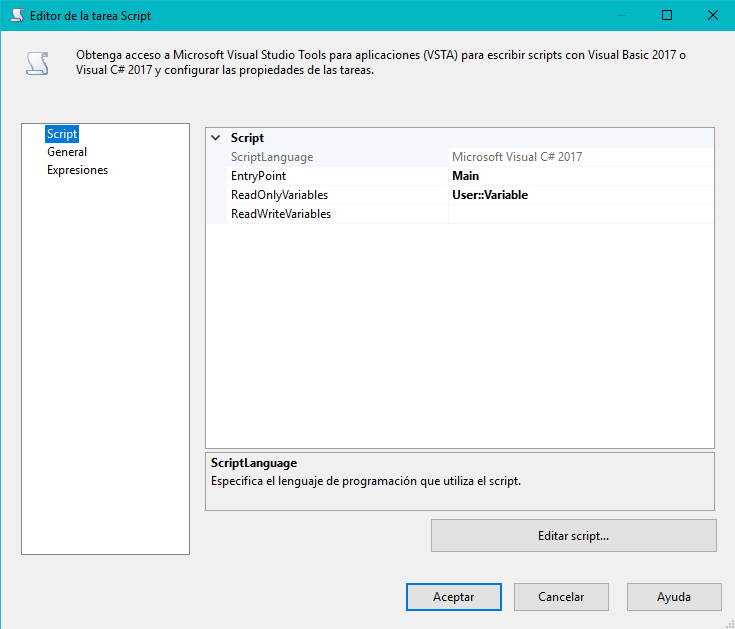
\includegraphics[width=13cm]{./Imagenes/img21}
	\end{center}	
9. El resultado obtenido .\\
	\begin{center}
	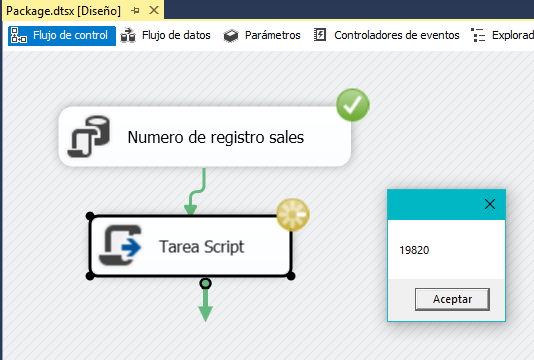
\includegraphics[width=14cm]{./Imagenes/img22}
	\end{center}	
10. Editamos una nueva tarea. \\
	\begin{center}
	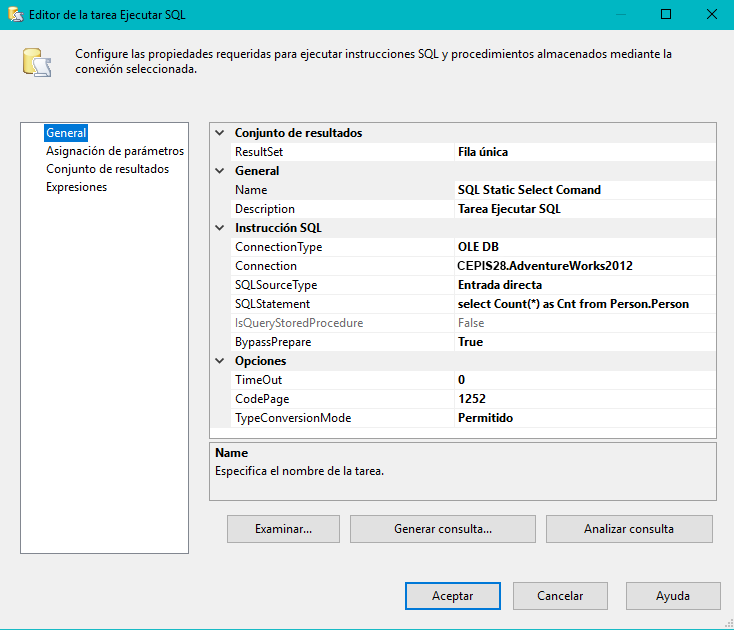
\includegraphics[width=12cm]{./Imagenes/img23}
	\end{center}	
11. Asignacion de parametros. \\
	\begin{center}
	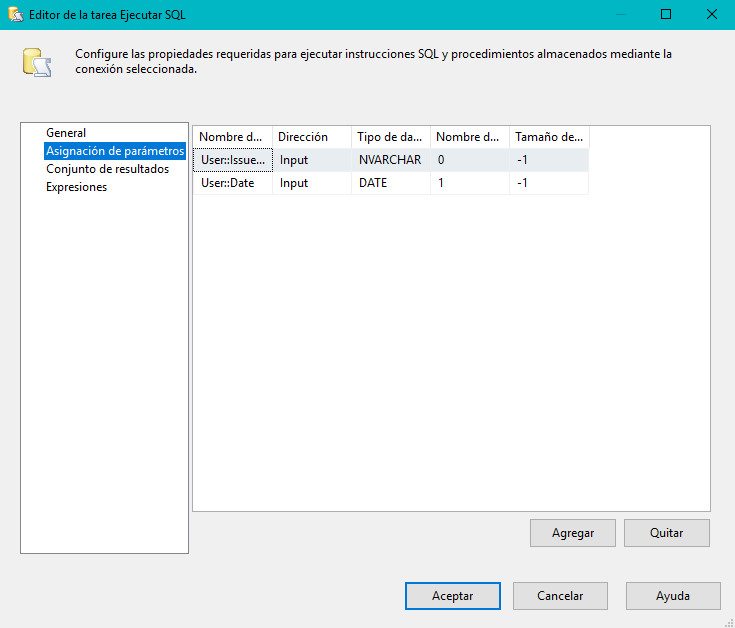
\includegraphics[width=12cm]{./Imagenes/img24}
	\end{center}	

	\begin{center}
	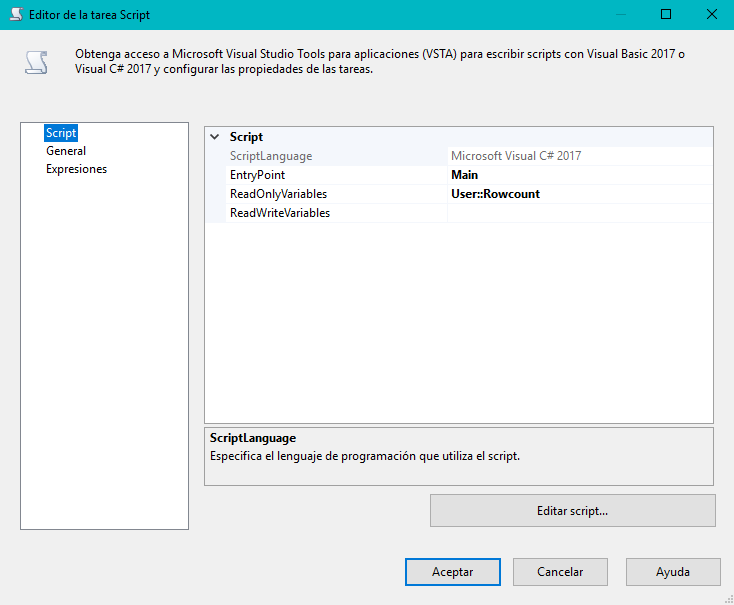
\includegraphics[width=12cm]{./Imagenes/img26}
	\end{center}	
12. Guardamos y los ejecutamos.\\
	\begin{center}
	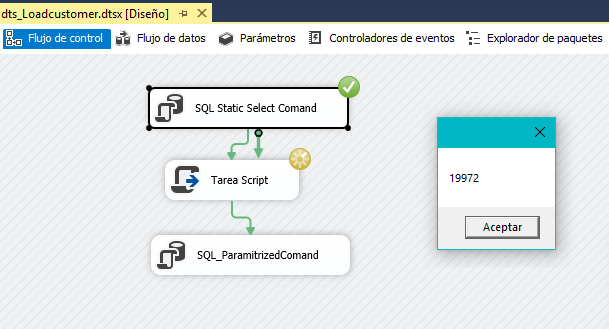
\includegraphics[width=15cm]{./Imagenes/img27}
	\end{center}	